\setNextFileName{ModifyingJikesRVM.html}
\begin{chapter}{Modifying Jikes RVM}
\label{cha:modifyingjikesrvm}

The sections \hyperref[sec:codingstyle]{Coding Style} and \hyperref[sec:codingconventions]{Coding Conventions} give a rough overview on existing coding conventions.

Jikes RVM is a bleeding-edge research project. You will find that some of the code does not live up to product quality standards. Don't hesitate to \href{http://www.jikesrvm.org/HowToHelp/}{help rectify this} by contributing clean-ups, refactorings, bug fixes, tests and missing documentation to the project.

\setNextFileName{AddingANewGarbageCollector.html}
\begin{section}{Adding a new garbage collector}
\label{sec:addinganewgarbagecollector}


\begin{subsection}{Overview}

This document describes how to add a new garbage collector to Jikes RVM.  We don't address how to design a new GC algorithm, just how to add a "new" GC to the system and then build it.  We do this by cloning an existing GC.  We leave it to you to design your own GC!

\end{subsection}

\begin{subsection}{Prerequisites}

Ensure that you have got a clean copy of the source (either a recent release or the hg tip) and can correctly and successfully build one of the base garbage collectors.  There's little point in trying to build your own until you can reliably build an existing one.  I suggest you start with MarkSweep, and that you use the \hyperref[sec:usingbuildit]{buildit} script:

\begin{lstlisting}
$ bin/buildit <targetmachine> BaseBase MarkSweep
\end{lstlisting}

Then test your GC:

\begin{lstlisting}
$ bin/buildit <targetmachine> -t gctest BaseBase MarkSweep
\end{lstlisting}

You should have seen some output like this:

\begin{lstlisting}
test:
     [echo] Test Result for [BaseBaseMarkSweep|gctest] InlineAllocation (default) : SUCCESS
     [echo] Test Result for [BaseBaseMarkSweep|gctest] ReferenceTest (default) : SUCCESS
     [echo] Test Result for [BaseBaseMarkSweep|gctest] ReferenceStress (default) : SUCCESS
     [echo] Test Result for [BaseBaseMarkSweep|gctest] FixedLive (default) : SUCCESS
     [echo] Test Result for [BaseBaseMarkSweep|gctest] LargeAlloc (default) : SUCCESS
     [echo] Test Result for [BaseBaseMarkSweep|gctest] Exhaust (default) : SUCCESS  
\end{lstlisting}

If this is not working, you should probably go and (re) read the section in the user guide on \hyperref[part:careandfeeding]{how to build and run} the VM.

\end{subsection}

\begin{subsection}{Cloning the MarkSweep GC}

 The best way to do this is in eclipse or a similar tool (see here for how to work with eclipse):
\begin{enumerate}
    \item Clone the \textit{org.mmtk.plan.marksweep as org.mmtk.plan.\textbf{mygc}}
      \begin{enumerate}
        \item You can do this with Eclipse:
          \begin{enumerate}
            \item Navigate to org.mmtk.plan.marksweep (within MMTk/src)
            \item Right click over org.mmtk.plan.marksweep and select "Copy"
            \item Right click again, and select "Paste", and name the target \newline org.mmtk.plan.mygc (or whatever you like)
            \item This will have cloned the marksweep GC in a new package called org.mmtk.plan.mygc
          \end{enumerate}
        \item or by hand:
          \begin{enumerate}
            \item Copy the directory MMTk/org/mmtk/plan/marksweep to \newline MMTk/org/mmtk/plan/mygc
            \item Edit each file within MMTk/org/mmtk/plan/mygc and change its package declaration to org.mmtk.plan.mygc
          \end{enumerate}
        \item We can leave the GC called "MS" for now (the file names will all be MMTk/org/mmtk/plan/mygc/MS*.java)
      \end{enumerate}
    \item Clone the BaseBaseMarkSweep.properties file as BaseBaseMyGC.properties:
      \begin{enumerate}
        \item Go to build/configs, and right click over BaseBaseMarkSweep.properties, and select "Copy"
        \item Right click and select "Paste", and paste as BaseBaseMyGC.properties
        \item Edit BaseBaseMyGC.properties, changing the text:
\begin{lstlisting}
config.mmtk.plan=org.mmtk.plan.marksweep.MS
\end{lstlisting}
to
\begin{lstlisting}
config.mmtk.plan=org.mmtk.plan.mygc.MS
\end{lstlisting}
      \end{enumerate}
    \item Now test your new GC:
\end{enumerate}
\begin{lstlisting}
$ bin/buildit <targetmachine> -t gctest BaseBase MyGC
\end{lstlisting}


You should have got similar output to your test of MarkSweep above.

That's it.  You're done. \smiley

\end{subsection}

\begin{subsection}{Making it Prettier}

You may have noticed that when you cloned the package \textit{org.mmtk.plan.marksweep}, all the classes retained their old names (although in your new namespace; \textit{org.mmtk.plan.\textbf{mygc}}).  You can trivially change the class names in an IDE like eclipse.  You can do the same with your favorite text editor, but you'll need to be sure that you change the references carefully.  To change the class names in eclipse, just follow the procedure below for each class in \textit{org.mmtk.plan.\textbf{mygc}}:
\begin{enumerate}
  \item Navigate to the class you want changed (eg  org.mmtk.plan.mygc.MS)
  \item Right click on the class (MS) and select \textit{"Refactor\textrightarrow\ Rename..."} and then type in your new name, (eg \textit{MyGC})
  \item Do the same for each of the other classes:
    \begin{itemize}
      \item MS \textrightarrow\  MyGC
      \item MSCollector \textrightarrow\  MyGCCollector
      \item MSConstraints \textrightarrow\  MyGCConstraints
      \item MSMutator \textrightarrow\  MyGCMutator
      \item MSTraceLocal \textrightarrow\  MyGCTraceLocal
    \end{itemize}
  \item Edit your configuration/s to ensure they refer to the renamed classes (since your IDE is unlikely to have done this automatically for you)
    \begin{itemize}
      \item Go to \textit{build/configs}, and edit each file \textit{*MyGC.properties} to refer to your renamed classes
    \end{itemize}
\end{enumerate}

\end{subsection}

\begin{subsection}{Beyond BaseBaseMyGC}

You probably want to build with configurations other than just BaseBase.  If so, clone configurations from MarkSweep, just as you did above (for example, clone \textit{FullAdaptiveMarkSweep} as \textit{FullAdaptive\textbf{MyGC}}). It's best to leave the Fast configurations for last, when you're sure that your GC is working correctly.

\end{subsection}

\begin{subsection}{What Next?}

Once you have this working, you have successfully created and tested your own GC without writing a line of code! You are ready to start the slightly more tricky process of writing your own garbage collector code.

If you are writing a new GC, you should definitely be aware of the \hyperref[cha:themmtktestharness]{MMTk test harness}, which allows you to test and debug MMTk in a very well contained pure Java environment, without the rest of Jikes RVM.  This allows you to write unit tests and corner cases, and moreover, allows you to edit and debug MMTk entirely from within your IDE.

\end{subsection}

\end{section}


\setNextFileName{CodingConventions.html}
\begin{section}{Coding Conventions}
\label{sec:codingconventions}

\begin{subsection}{Assertions in Jikes RVM and MMTk}

Partly for historical reasons, we use our own built-in assertion facility rather than the one that appeared in Sun®'s JDK 1.4. All assertion checks have one of the two forms:

\begin{lstlisting}[language=Java]
if (VM.VerifyAssertions)  VM._assert(condition)
if (VM.VerifyAssertions)  VM._assert(condition,  message)
\end{lstlisting}

\spverb+VM.VerifyAssertions+ is a \spverb+public static final+ field. The \texttt{con\-fig.as\-ser\-tions} configuration variable determines \spverb+VM.VerifyAssertions+' value. If \texttt{con\-fig.as\-ser\-tions} is set to none, Jikes RVM has no assertion overhead.

If you use the form without a message, then the default message "vm internal error at:" will appear.

If you use the form with a message the message must be a single string literal. Doing string appends in assertions can be a source of horrible performance problems when assertions are enabled (i.e. most development builds). If you want to provide a more detailed error message when the assertion fails, then you must use the following coding pattern:

\begin{lstlisting}[language=Java]
if (VM.VerifyAssertions && condition) {
  ... build message ...
  VM._assert(VM.NOT_REACHED, message);
}
\end{lstlisting}

An assertion failure is always followed by a stack dump.

Use \spverb+VM.ExtremeAssertions+ instead of \spverb+VM.VerifyAssertions+ if the assertion is costly to check but generally useful. These kinds of assertions are only enabled when \spverb+config.assertions+ is set to \spverb+extreme+.

Use \spverb+IR.SANITY_CHECK+ or \spverb+IR.PARANOID+ to guard assertions that relate to the intermediate representation in the optimizing compiler.

\end{subsection}

\begin{subsection}{Assertions in the MMTk Test Harness}

The assert keyword may be used in the MMTk Harness.

\end{subsection}

\begin{subsection}{Error Handling}

All code in the system needs to detect and handle errors. If you know that your code does not handle certain situations, you should aim to write the code in way that detects these situations. The code also needs to be documented well enough so that users get a hint about the source of the problem. Keep in mind that the Jikes RVM is also used by students who may not be as familiar with the domain as researchers are.

\begin{subsubsection}{Examples}
  \begin{itemize}
    \item The code does not work at all in a certain situation, e.g. it gives incorrect results when the optimizing compiler is enabled or a certain optimization is turned on. In this case, the best approach is to detect the situation and fail fast. This can be done using assertions. You can use VM.sysFail(..) for builds without assertions if correct execution after failure is impossible.
    \item A compiler optimizations fails. The correct approach is to throw an OptimizingCompilerException (e.g. via one of the static methods provided by that class). This will lead to a hard failure when -X:vm:errorsFatal=true is set (which is the case in regression tests). In other cases, the VM will just revert to using the baseline compiler.
    \item A command line option has a limited range of values. In MMTk, the correct approach is to implement the validate() method for the option. In other places, the value of the option needs to be checked at a suitable time.
  \end{itemize}
\end{subsubsection}

\end{subsection}
 

\end{section}


\setNextFileName{CodingStyle.html}
\begin{section}{Coding Style}
\label{sec:codingstyle}

Regrettably, some code in the current system does not follow any consistent coding style. This is an unfortunate residuum of the system's evolution.

We use checkstyle to support a gradually expanding subset of coding conventions.  The current set of enforced checkstyle rules are defined by \texttt{\$RVM\_ROOT/build/check\-style/rvm-checks.xml} and are verified as part of the pre-commit test run. To check for violations of the coding style without running the tests, \hyperref[sec:usingbuildit]{use buildit} or run "ant checkstyle" from the command line.

\begin{subsection}{File Headers}

Every file needs to have the license header.

A Java example of the notices follows.

\begin{lstlisting}[language=Java]
/*
 *  This file is part of the Jikes RVM project (http://jikesrvm.org).
 *
 *  This file is licensed to You under the Eclipse Public License (EPL);
 *  You may not use this file except in compliance with the License. You
 *  may obtain a copy of the License at
 *
 *      http://www.opensource.org/licenses/eclipse-1.0.php
 *
 *  See the COPYRIGHT.txt file distributed with this work for information
 *  regarding copyright ownership.
 */
package org.jikesrvm;

import org.jikesrvm.classloader.ClassLoader; // FILL ME IN

/**
 * TODO Substitute a brief description of what this program or library does.
 */
\end{lstlisting}

\end{subsection}

\begin{subsection}{Coding style description}

The Jikes\textsuperscript{TM} RVM coding style guidelines are similar to the Sun® Microsystems "Code Conventions for the Java\textsuperscript{TM} Programming Language", with a few exceptions listed below. Most of the style guide is intuitive; however, please read through the document (or at least look at its sample code).

We have adopted four modifications to the Sun code conventions:

\begin{itemize}
  \item \textbf{Two-space indenting} The Sun coding convention suggests 4 space indenting; however with 80-column lines and four-space indenting, there is very little room left for code. Thus, we recommend using 2 space indenting. There are to be no tabs in the source files or trailing white space on any line.
  \item \textbf{132 column lines in exceptional cases} The Sun coding convention is that lines be no longer than 80 columns. Several Jikes RVM contributors have found this constraining. Therefore, we allow 132 column lines for exceptional cases, such as to avoid bad line breaks.
  \item \spverb+if (VM.VerifyAssertions)+ As a special case, the condition \texttt{if \newline (VM.VerifyAssertions)} is usually immediately followed by the call to \spverb+VM._assert()+, with a single space substituting for the normal newline-and-indentation. See the \hyperref[sec:codingconventions]{coding conventions} for an example.
  \item \textbf{Capitalized fields} Under the Sun coding conventions, and as specified in The Java Language Specification, Second Edition, the names of fields begin with a lowercase letter. (The only exception they give is for some final static constants, which have names \spverb+ALL_IN_CAPITAL_LETTERS+, with underscores separating them.) That convention reserves IdentifiersBeginningWithACapitalLetterFollowedByMixedCase for the names of classes and interfaces. However, most of the final fields in the Configuration class and the Properties interface also are in that format. Since the VM class inherits fields from both Properties and Configuration, that's how we get VM.VerifyAssertions, etc.
\end{itemize}

\end{subsection}

\begin{subsection}{Javadoc requirements}

All non-trivial files should contain descriptive comments in \href{http://www.oracle.com/technetwork/java/javase/documentation/index-jsp-135444.html}{Javadoc\textsuperscript{TM}} form so that documentation can be generated automatically. Of course, additional non-Javadoc source code comments should appear as appropriate.
\begin{enumerate}
  \item Classes, methods and fields should have a block comment describing them if it makes sense. There is no need to add comments merely for the sake of commenting. For example, it is not necessary to add a comment for a method if the comment does not provide more information than the signature and the method name already do.
  \item JavaDoc comments must not be copied from methods that are being overriden. If the comment from the method that you are overriding is sufficient, you do not need to provide JavaDoc for the newly added method - JavaDoc will automatically copy the JavaDoc from the overriden method. If you want to extend the comment from the overriden method with new information, use {@inheritDoc} to copy the comment from the superclass and add your text.
  \item JavaDoc for methods contains a short description of their arguments (using \spverb+@param+), the return value (using \spverb+@return+) and the exceptions they may throw (using \spverb+@throws+).
  \item Each class should include \spverb+@see+ and \spverb+@link+ references as appropriate.
\end{enumerate}
\end{subsection}

\end{section}


\setNextFileName{CompilerDNA.html}
\begin{section}{Compiler DNA}
\label{sec:compilerdna}

The Jikes RVM adaptive system uses the compiler DNA found in \newline \spverb+org.jikesrvm.adaptive.recompilation.CompilerDNA+. The important values in here are the \spverb+compilationRates+ and the \spverb+speedupRates+. If you modify Jikes RVM then it's likely you need to recalibrate the adaptive system for your changes.

In Jikes RVM 3.1.3 or earlier, do the following:

\begin{enumerate}
    \item run the compiler-dna test harness ("ant -f test.xml -Dtest-run.name=compiler-dna"). This will automatically compile and run Jikes RVM on SPEC JVM '98. You will want to configure the ant property external.lib.dir to be a directory containing your SPEC JVM '98 directory. Your SPEC JVM '98 directory must be named "SPECjvm98".
    \item load the xml file \spverb+results/tests/compiler-dna/Report.xml+ into either an XML viewer (such as a web browser) or into a text editor
    \item find the section named \spverb+Measure_Compilation_Base+, then look within this section for statistics and find the static Base.bcb/ms. For example, \spverb+<statistic key="Base.bcb/ms" value="1069.66"/>+. In the \newline \spverb+compilationRates+ array this will be the value of element 0, it corresponds to how many bytecodes the baseline compiler can compile per millisecond.
    \item find the section named \spverb+Measure_Compilation_Opt_0+ and the statistic Opt.bcb/ms. This is element 1 in the \spverb+compilationRates+ array.
    \item find the section named \spverb+Measure_Compilation_Opt_1+ and the statistic Opt.bcb/ms. This is element 2 in the \spverb+compilationRates+ array.
    \item find the section named \spverb+Measure_Compilation_Opt_2+ and the statistic Opt.bcb/ms. This is element 3 in the \spverb+compilationRates+ array.
    \item find the section named \spverb+Measure_Performance_Base+ and the statistic named \spverb+aggregate.best.score+ and record its value. For example, for \spverb+<statistic key="aggregate.best.score" value="28.90"/>+ you would record 28.90.
    \item find the section named \spverb+Measure_Performance_Opt_0+ and the statistic \spverb+named aggregate.best.score+. Divide this value by the value you recorded in step 7, this is the value for element 1 in the \spverb+speedupRates+ array. For example, for \spverb+<statistic key="aggregate.best.score" value="137.50"/>+ the \spverb+speedupRates+ array element 1 should have a value of 4.76.
    \item find the section named \spverb+Measure_Performance_Opt_1+ and the statistic named \spverb+aggregate.best.score+. As with stage 8 divide this value by the value recorded in step 7, this is the value for element 2 in the \spverb+speedupRates+ array.
    \item find the section named \spverb+Measure_Performance_Opt_2+ and the statistic named \spverb+aggregate.best.score+. As with stage 8 divide this value by the value recorded in step 7, this is the value for element 3 in the \spverb+speedupRates+ array.
\end{enumerate}

In Jikes RVM 3.1.4 or later, the directory for the test results (e.g. \newline \spverb+results/tests/compiler-dna/+) should contain a file \spverb+CompilerDNA.xml+. Copy the contents into \spverb+CompilerDNA+ and modify them so that the code compiles.

You should then save \spverb+CompilerDNA+ and recompile a production RVM which will use these values.

If you are frequently changing the compiler dna, you may want to use the command line option \spverb+-X:aos:dna=<file name>+ to dynamically load compiler dna data without having to rebuild Jikes RVM.


\end{section}


\setNextFileName{EditingJikesRVMInAnIDE.html}
\begin{section}{Editing Jikes RVM in an IDE}
\label{sec:editingjikesrvminanide}

One goal of the JikesRVM project over recent years has been the ability to develop Jikes RVM in a development environment such as Eclipse. This has been possible for the MMTk component since 2005, and as of early 2007 (release 2.9.0) it is possible to work with the majority of the Jikes RVM codebase in Eclipse and similar environments.  With Jikes RVM release 2.9.1, setting up your Eclipse environment to work with Jikes RVM became even easier.

\begin{subsection}{Editing JikesRVM in Eclipse}

These instructions assume you are working with Jikes RVM version 2.9.1 or later.

\begin{enumerate}
  \item Create a JikesRVM source tree either via Git checkout or unpacking a distribution.
     \begin{lstlisting}
$ git clone https://github.com/JikesRVM/JikesRVM.git
     \end{lstlisting}
  \item Create the machine-generated files and eclipse metadata:
     \item If you have a recent version of Jikes RVM (3.0 onwards):
       \begin{lstlisting}
$ cd jikesrvm
$ bin/buildit --eclipse localhost
       \end{lstlisting}
        \textit{Note that if you will not or cannot build on your local machine}, substitute localhost for the name of a host you can build on (buildit will perform the build remotely and then copy the requisite files back).

     \item If you are working on an older version (2.9.1 - 2.9.3), you can follow this procedure:
       \begin{lstlisting}
$ cd jikesrvm
$ ant -Dhost.name=ia32-linux -Dconfig.name=development
$ ant -Dhost.name=ia32-linux -Dconfig.name=development eclipse-project
       \end{lstlisting}
        If you will not or cannot build on your local machine:
       \begin{enumerate}
         \item copy your tree to build build host somehow
         \item perform the above ant tasks
         \item copy the following generated files and directories back to the machine you will edit on:
           \begin{itemize}
             \item jikesrvm/.project
             \item jikesrvm/.classpath
             \item jikesrvm/eclipse
           \end{itemize}
       \end{enumerate}
  \item Import the newly created Eclipse project into your Eclipse workspace.
    \begin{enumerate}
      \item From Eclipse, select File \textrightarrow\ Import
      \item Select "Existing Projects Into Workspace"
        \begin{figure}[h]
          \centering
          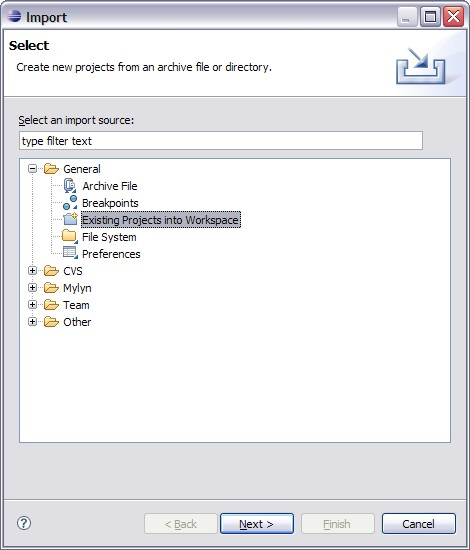
\includegraphics[width=\textwidth]{images/EditingJikesRVMInAnIDE-ImportProject.jpg}
        \end{figure}
      \item Browse to find the top-level directory.
      \item Select the project (in this case JikesRVM ia32-linux development)
        \begin{figure}[h]
          \centering
          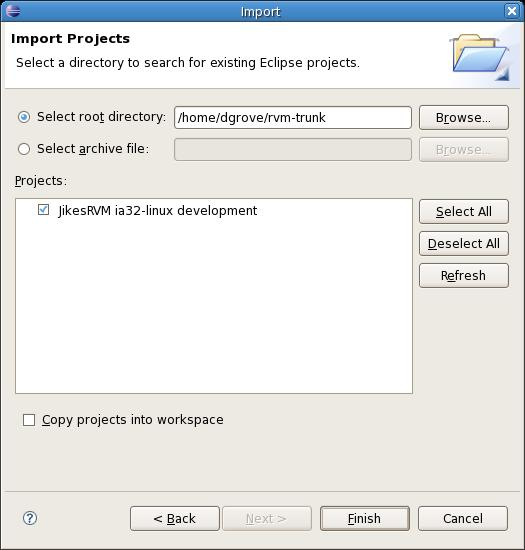
\includegraphics[width=\textwidth]{images/EditingJikesRVMInAnIDE-SelectDirectory.jpg}
        \end{figure}
      \item Hit Finish
    \end{enumerate}
\end{enumerate}

\end{subsection}

\begin{subsection}{Setup for easier compliance with the Checkstyle rules}

If you consider \href{http://www.jikesrvm.org/Contributions/}{contributing} changes back to Jikes RVM, it is helpful to configure your IDE to comply with the Jikes RVM \hyperref[sec:codingstyle]{coding style}. The coding style forbids the use of tabs and requires that no line ends with whitespace.

If you have a separate workspace for your work with Jikes RVM, you can set up Eclipse for correct tab usage by configuring the text editors. Go to Window \textrightarrow\ Preferences and then to General \textrightarrow\ Editors \textrightarrow\ Text editors (Eclipse 3.6) or Window \textrightarrow\ Preferences \textrightarrow\ General \textrightarrow\ Editors \textrightarrow\ Text Editors (Eclipse 3.5 and earlier). Check "Insert spaces for tabs". Make sure that "Displayed tab width" is set to 2. This setting affects the non-Java editors (e.g. XML editor for the ant files for the build).

To set the tab width for Java code, you need to setup the Java code style. We currently do not provide a style template, so you will have to define your own. Go to the project properties (e.g. via Project \textrightarrow\ Properties) and select Java Code Style \textrightarrow\ Formatter. Check the box "Enable project specific settings" and create a new profile for Jikes RVM. Edit the new profile. In the edit dialog, choose the tab "Indentation". Set the tab policy to "Spaces only" and set both indentation size and tab size to 2. Also make sure that the box "Empty lines" at the bottom of the "Indentation" tab is not checked.

To ensure that you do not introduce whitespace at the end of lines you can configure Eclipse's Save actions in the project properties at Java Editor \textrightarrow\ Save Actions. Check the box "Enable project specific settings" and the box "Perform the selected actions on save" as well as "Additional actions". Press "Configure" and check the box "Remove trailing whitespace" in the "Code Organizing" tab.

\end{subsection}

\begin{subsection}{Editing JikesRVM in NetBeans}

\begin{enumerate}
  \item Follow the instructions for Eclipse including building the eclipse project with ant
  \item Install the Eclipse project importer
  \item Select File \textrightarrow\ Import Project \textrightarrow\ Eclipse Project
    \begin{enumerate} 
      \item Choose to import project ignoring project dependencies
      \item Select the top-level directory you created with the JikesRVM in as the project to import
      \item Select a new folder as the destination (workspace) for the import
      \item Hit Finish
    \end{enumerate}
\end{enumerate}

\end{subsection}

\end{section}


\end{chapter}
